%!TEX program = lualatex
\documentclass[a4paper, 11pt]{scrartcl}

\usepackage{csquotes}
\usepackage{kpfonts}
\usepackage[hidelinks]{hyperref}

% Code Segments
\usepackage{listings}
% Copyright 2017 Sergei Tikhomirov, MIT License
% https://github.com/s-tikhomirov/solidity-latex-highlighting/

\usepackage{listings, xcolor}

\colorlet{punct}{red!60!black}
\definecolor{background}{HTML}{EEEEEE}
\definecolor{delim}{RGB}{20,105,176}
\colorlet{numb}{magenta!60!black}

\lstdefinelanguage{json}{
    basicstyle=\normalfont\ttfamily,
    numbers=left,
    numberstyle=\scriptsize,
    stepnumber=1,
    numbersep=8pt,
    showstringspaces=false,
    breaklines=true,
    frame=lines,
    backgroundcolor=\color{background},
    literate=
     *{0}{{{\color{numb}0}}}{1}
      {1}{{{\color{numb}1}}}{1}
      {2}{{{\color{numb}2}}}{1}
      {3}{{{\color{numb}3}}}{1}
      {4}{{{\color{numb}4}}}{1}
      {5}{{{\color{numb}5}}}{1}
      {6}{{{\color{numb}6}}}{1}
      {7}{{{\color{numb}7}}}{1}
      {8}{{{\color{numb}8}}}{1}
      {9}{{{\color{numb}9}}}{1}
      {:}{{{\color{punct}{:}}}}{1}
      {,}{{{\color{punct}{,}}}}{1}
      {\{}{{{\color{delim}{\{}}}}{1}
      {\}}{{{\color{delim}{\}}}}}{1}
      {[}{{{\color{delim}{[}}}}{1}
      {]}{{{\color{delim}{]}}}}{1},
}

\lstset{
  language=json,
  escapeinside={<@}{@>},
	backgroundcolor=\color{verylightgray},
	extendedchars=true,
	basicstyle=\footnotesize\ttfamily,
	showstringspaces=false,
	showspaces=false,
	numbers=left,
	numberstyle=\footnotesize,
	numbersep=9pt,
	tabsize=2,
	breaklines=true,
	showtabs=false,
	captionpos=b
}


% Images
\usepackage{graphicx}

% Sequence Diagram
\usepackage{geometry}
\usepackage{pgf-umlsd}
\usetikzlibrary{calc}

% Glossary
\usepackage[toc,section=section]{glossaries}
\makeglossaries
\usepackage{glossaries}


\newacronym{utc}{UTC}{Coordinated Universal Time}
\newacronym{adt}{ADT}{Atlantic Daylight Time}
\newacronym{est}{EST}{Eastern Standard Time}
\newglossaryentry{fido2}{name=FIDO2, description=New standart from the FIDO Alliance which combines CTAP and WebAuthn}
\newacronym{fido}{FIDO}{Fast IDentity Online}
\newacronym{ctap}{CTAP}{Client-to-Authenticator Protocol}
\newacronym{nist}{NIST}{National Institute of Standards and Technology}
\newacronym{webAuthn}{WebAuthn}{Web Authentication}
\newacronym{u2f}{U2F}{Universal 2nd Factor}
\newacronym{rest}{REST}{REpresentional State Transfer}
\newacronym{api}{API}{Application Programming Interface}
\newacronym{json}{JSON}{JavaScript Object Notation}
\newacronym{cose}{COSE}{CBOR Object Signing and Encryption (COSE)}
\newacronym{cbor}{CBOR}{Concise Binary Object Representation}
\newglossaryentry{sha-256}{name=SHA-256, description=Secure Hash Algorithm 2 with 256 Bit Output}
\newacronym{utf-8}{UTF-8}{Universal Transofmation Format}
\newacronym{nfc}{NFC}{Near Field Communication}
\newacronym{usb}{USB}{Universal Serial Bus}
\newacronym{eid}{eID}{electronical IDentity}
\newacronym{hlos}{HLOS}{High Level Operating System}
\newacronym{aroe}{AROE}{Allowed Restricted Operating System}
\newacronym{mitm}{MitM}{Man in the Middle}
\newacronym{}{}{}


\usepackage{polyglossia}
\setdefaultlanguage{english}
\usepackage[backend=biber, style=ieee]{biblatex}
\addbibresource{paper.bib}
\usepackage{graphicx}
\begin{document}
\title{Web Authn Reference Implementation}
\date{\today} 
\author{ Julian Stampfli (\texttt{julianjimmy.stampfli@students.bfh.ch}) }
\maketitle
\setcounter{tocdepth}{2}
\tableofcontents
\clearpage

\section{Introduction}

Passwords are the most commonly used way to authenticate a user. They are easy to implement and have been used since the beginning of the internet. People are used to passwords and use them everywhere, but most of them use weak ones. Remembering strong passwords is not easy; thus, most opt for easier passwords or reuse them. The newest recommendations from the \gls{nist} are to use very long passwords that make sense for a human but are hard to guess for a computer — for instance a sentence in a fictional language or with slang or unusual words. An appropriate password would then look something like `awsumfurrycybercat', but not that\cite{nist:pw:blog, nist:pw}.

But even when user employ strong passwords, it is hard to remember a new password for every site. Thus, they tend to reuse passwords for multiple sites. Password reuse can lead to \gls{csa}\cite{panda:pwreuse, xkcd:pwreuse}.

Those are two weaknesses that passwords always had. Firstly, used passwords are generally too weak; secondly, they same are used for multiple services. 

\gls{fido2} is a specification that aims to increase security for end users by eliminating the weaknesses that come with passwords. The main advantages are strong privacy, privacy protection, multiple choices, cost-efficiency, and a layered approach. It tries to do that by using secure authenticators instead of a password.  Additionally to the already discussed attacks \gls{fido2} also protects against \gls{mitm} attacks\cite{yubico:whatIsFido2}.

The main force behind \gls{fido2} is the \gls{fido} Alliance. Some notable members are Microsoft, Google, and Yubico. Microsoft, for instance, wants to use \gls{fido2} for the Windows Hello login\cite{yubico:ms}. With the force behind the standard, it is implemented in all major web browser\cite{fido:browser}. There are also already authenticators available from Yubico, and possibly others, that can support it\cite{yubico:yubikey5}.

This paper discusses the implementation for the \gls{rp} when the user already has a \gls{fido2} authenticator.

\section{FIDO2}

\gls{fido2} is an authentication standard which uses public key cryptography to authenticate the user. Compared to a password the user doesn't prove that he knows something but that he has something which he previously has registered with the application. It is also possible to secure this authenticator with a second factor like a pin or biometrics. The authenticator is an external device that interacts with the application through a protocol called \gls{ctap}. \gls{ctap} is also part of the \gls{fido2} specification but this paper does not go into detail about how this protocol works\cite{ctap}.

The \gls{webAuthn} specification forms the second part of \gls{fido2}. This part deals with the Application that wants to authenticate the user. It contains two steps. Attestation which deals with registering a new user and assertion which handles the authentication of an existing user. Both functions are explained in Section \ref{sec:replying_party}.

\subsection{Main Ideas}

Traditionally, when a user wants to register or authenticate, he supplies the application with a password. A shared secret that only the user is supposed to know. We already discussed how passwords usually lead to weak authentication. This issue is normally circumvented by adding a second factor to the authentication. With \gls{fido} \gls{u2f} this second factor would be robust, and the authentication would be resilient against scaled attacks. However, many sites offer weaker forms of second-factor authentication like codes via e-mail or SMS. Both of those methods are weak to message interception\cite{smsweak}.

In \gls{fido2} the Authenticator receives a challenge when it is accessed. This challenge comes from the \gls{rp} which wants to authenticate a user. With the challenge, the \gls{rp} sends the domain name where it is available. The authenticator can then check if that is truly the domain where the user is accessing the site. Should this be valid, the authenticator creates a response by signing the challenge and the host. The \gls{rp} can then check whether the challenge and the domain contain the requested values and whether the signature is correct. With this, a \gls{mitm} attacker can't forward a challenge from a \gls{rp} to an authenticator by using a spoofed page. The user and the \gls{rp} can both be assured that they are talking to the correct party. To assure this \gls{tls} is mandatory for each session\cite{yubico:whatIsFido2}.

By using certified authenticators, \gls{fido2} makes sure that a user needs to have access to his authenticator and be present when the authentication is triggered. With this, an attacker could still steal the physical authenticator and authenticate with it. However, this kind of physical attack can't be used to steal the authenticators for a large group of people and thus doesn't scale. Additionally, once the user notices that his authenticator has been stolen, he can inform the service provider and disable this authenticator for future authentications. Moreover, authenticators that are left plugged into the machine are also secured by this mechanism. An attacker that wants to remotely trigger the authentication can't get the user present flag to be active even if the authenticator is left in the machine for a long time. 

\subsection{Authenticator}
\gls{fido2} authenticators are certified devices that support the \gls{fido2} standard. They must at least fulfill level 1 of the certification levels. 4 levels can be achieved that all build on each other. New authenticators need first to get a functional certificate to prove that they are interoperable with other clients and servers and thus fulfill the \gls{fido2} standard.

The authenticator used in this reference implementation is a Yubikey 5 which offers an interface for \gls{fido2} via \gls{usb} and via \gls{nfc}. In this paper, only the \gls{usb} interface is used.

\subsubsection{Level 1}
Level 1 is the basic level. It offers protection against basic, at-scale attacks\cite{fido:authenticator:level1}.

This level can range from an authenticator running in a \gls{hlos} without effective protection against most other applications to an authenticator being implemented completely in an \gls{aroe}. Most authenticators that are used should belong to a security level above 1 to ensure the security of the authenticator and the authentication\cite{fido:authenticator:level1}.

\subsubsection{Level 2}
Level 2 protects against basic, scalable attacks\cite{fido:authenticator:level2}.

This level needs an authenticator to run in a \gls{fido} \gls{aroe} and needs to support allowed cryptography lists. Examples that would not achieve this level are\cite{fido:authenticator:level2, fido:authenticator:allowedEnvironment}:
\begin{enumerate}
  \item Authenticator that doesn't support attestation
  \item Authenticator that is an implementation without a restricted operating environment 
\end{enumerate}

\subsubsection{Level 3}
Level 3 protects against enhanced-basic effort software and hardware attacks. The \gls{fido} alliance provides some examples that would pass level 3\cite{fido:authenticator:level3}.

Some simplified examples are:
\begin{enumerate}
  \item Authenticator that can't be easily opened implemented on a CPU with RAM encryption and integrity check.
\end{enumerate}

\subsubsection{Level 3+}
Level 3+ protects against moderate or high effort software or hardware attacks. Thus an attacker should be hindered from performing attacks on a chip level\cite{fido:authenticator:level3_plus}.

\subsection{FIDO2 vs FIDO U2F}

\gls{fido} \gls{u2f} is the predecessor of \gls{fido2}. \gls{fido2} covers more usecases than \gls{fido} \gls{u2f}. \gls{fido} \gls{u2f} is only for second factor authentication, \gls{fido2} can be used as a second factor but also for passwordless authentication and local multifactor authentication\cite{yubico:whatIsFido2}.

Another major difference is the location of the private keys. In \gls{fido} \gls{u2f} it is possbile to store the private key in the key handle on the server in an encrypted form. This makes it easy to access a lot of services with the same authenticator because the authenticator doesn't need to store anything. However, the security of this approach is questionable. With \gls{fido2} the private keys never leave the authenticator\cite{fido:u2fImplementationConsiderations, fido:howitworks}.

It is possible to use a \gls{fido} \gls{u2f} token to authenticate with a \gls{fido2} \gls{rp} and vice verca. This mapping is mainly done in the \gls{ctap} version 1 for \gls{fido} \gls{u2f} and version 2 for \gls{fido2}. In the \gls{fido2} version there is a mapping defined which can map a response of a \gls{fido} \gls{u2f} authenticator to a response of a \gls{fido2} authenticator. This mapping for the authentication can be seen in Figure \ref{fig:authenticationMapping}. The full description is available in the \gls{ctap} specification\cite{yubico:whatIsFido2, ctap:interoperability}.

\begin{figure}[ht]
  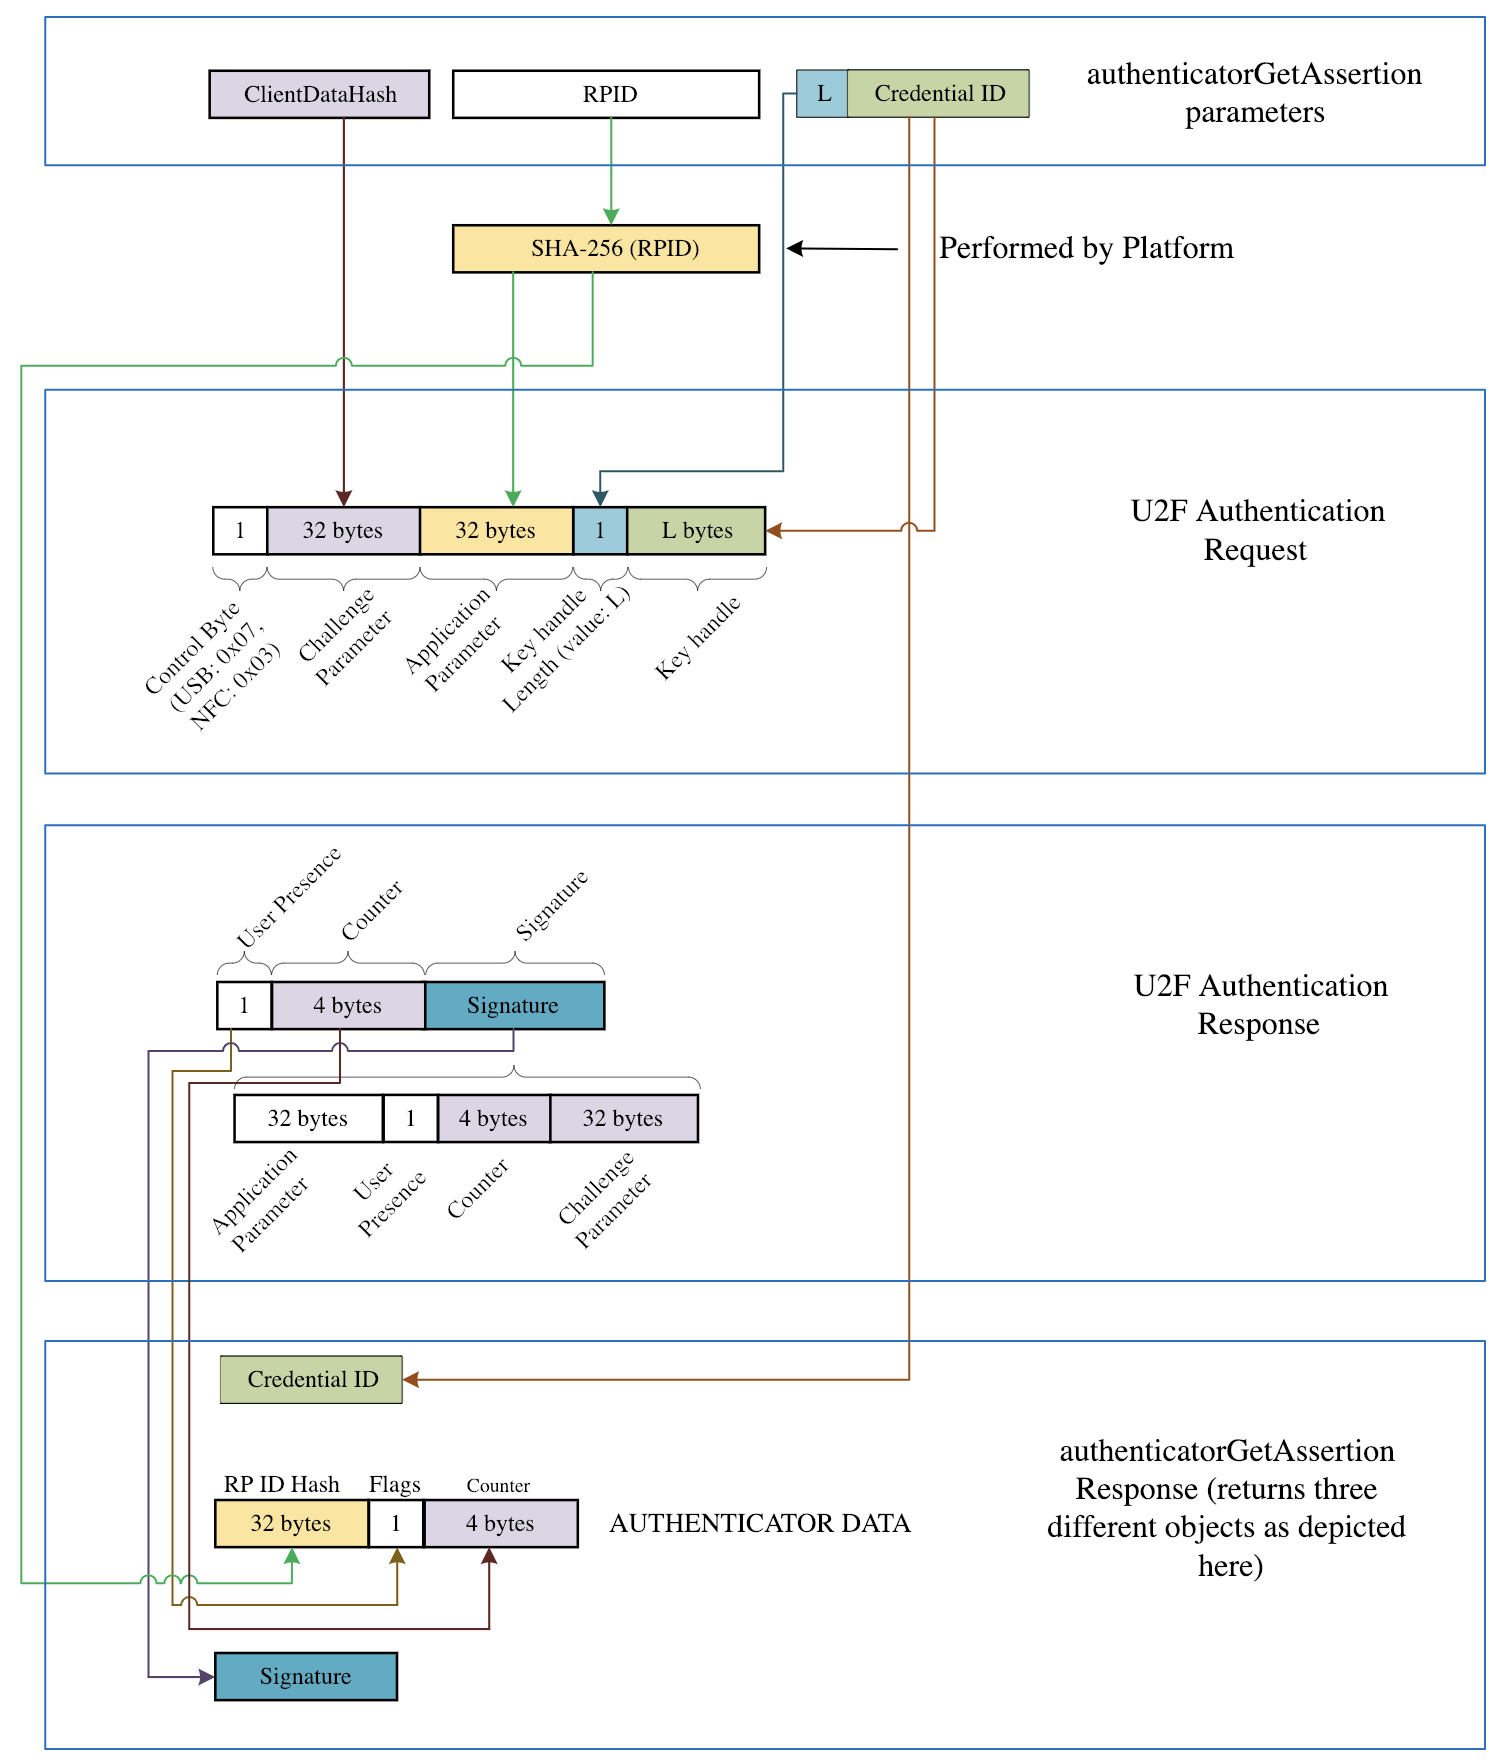
\includegraphics[width=16cm]{img/u2fcompat-getassertion.png}
  \centering
  \caption{Authenticator Data}
  \label{fig:authenticationMapping}
\end{figure}


\section{Relying Party Reference Implementation}
\label{sec:replying_party}

The \gls{rp} is one of the main components of the \gls{webAuthn} standard and the main component of this paper. It includes a sample implementation of the \gls{rp} meant as a reference. This part deals with the two phases attestation and authentication. First, there is a short section dealing with the setup of the reference code.

\subsection{Environment}

The reference code is written in Java and uses Maven for dependency management. To get the \gls{rest} \gls{api} set up Spring Boot is used such that most of the non-relevant code isn't needed. The data from the registrations are stored in a set to decrease the non-relevant code even more. Additionally, there are some data classes which are used within the application.

The frontend part is from the \gls{fido} Alliance demo\cite{fido:demo}. Additionally, some inspiration was taken from the Yubico implementation of the Java-Webauthn-Server also available on Github\cite{yubico:webauthn:server}. 

For testing the YubiKey 5 was used\cite{yubico:yubikey5} which is reflected in the code. There are multiple ways with which the standard can be implemented. Only the way to implement it with a Yubikey 5 is available in the reference code. The other ways are discussed in their paragraphs.

The most important classes are the LoginController, the RegistrationController, and the AuthenticatorDataParser. Those are supposed to be references for when one wants to implement the \gls{rp} oneself. Those classes are discussed in depth in the following sections.

For testing the \gls{rp} it is important to generate a valid certificate and to communicate with a valid domain. If the \gls{rp} listens to localhost the response is invalid. The same happens when the communication is not secured with a valid certificate and in a \gls{tls} connection.

\clearpage

\subsection{Registration / Attestation}

The registration which is reflected in the RegistrationController represents the process a user has to go through to register with the application using a \gls{fido2} authenticator. It consists of two main steps. First, the \gls{rp} has to create a \gls{json} that is accepted by the token in the \gls{ctap} protocol as a valid challenge. After the response from the client, the response endpoint needs to validate the input from the authenticator. This can be seen in Figure \ref{fig:user_registration}.

\begin{figure}[h]
  \centering
  \begin{sequencediagram}
    \newthread{U}{User}{}
    \newinst[1]{T}{Authenticator}{}
    \newinst[2.5]{B}{Browser}{}
    \newinst[3]{R}{\gls{rp}}{}
    \begin{call}{U}{Register}{B}{}
      \begin{call} {B}{/create(user)}{R}{makeCredentialJson}
      \end{call} 
      \begin{call} {B}{webAuthn.create}{T}{createResponse}
        \begin{call}{T}{activate}{U}{activation}
        \end{call}
      \end{call} 
      \begin{call} {B}{/response(createResponse)}{R}{username}
      \end{call} 
    \end{call}
  \end{sequencediagram}
  \caption{User Registration}
  \label{fig:user_registration}
\end{figure}

\subsubsection{Create registration}

The create registration step consists of creating a \gls{json} which represents a valid challenge. This \gls{json} is sent to the browser where it is handed to the call `navigator.create()'. The response is sent to the /response endpoint in the \gls{rp}.

A valid \gls{json} representation of this response can be seen in Listing \ref{lst:createRegistration}. A description to the important entries follows:

\lstinputlisting[language=json, caption=Registration \gls{json}, label=lst:createRegistration]{json/createRegistration.json}

\begin{description}
  \item[challenge] \hfill \\ The challenge to be signed by the Authenticator. Must be unique for each call and \gls{base64} encoded.
  \item[fidoResponse] Should be `direct'. 
  \item[rp.id] \hfill \\ Must reflect the domain over which you communicate
  \item[user.id] Must be unique and random. 
  \item[pubKeyCredParams.type] Should be `public-key'. 
  \item[pubKeyCredParams.alg] Must be a valid \gls{cose} algorithm\cite{cose}.
  \item[attestation] Should be `direct'.
  \item[timeout] Should be defined.   
\end{description}


\subsubsection{Verify registration}

To verify the response of an authenticator the specification provided 19 steps. The implementation closely followed those steps by creating a method for each. If something went wrong it will throw an exception and return with an error code. The following paragraphs will provide some further documentation and challenges that were faced while implementing the reference. The initial response can be seen in Listing \ref{lst:create_response}.

\lstinputlisting[language=json, caption=Create Response \gls{json}, label=lst:create_response]{json/createResponse.json}

\paragraph{Step1} \hfill \\ 
In Java with Spring Boot, the first step is mostly not needed. But the check that the needed fields in the \gls{json} are present can be done at this point.

\paragraph{Step2} \hfill \\ 
In step 2 the `clientDataJSON' field has to be parsed. This is done by \gls{base64} URL decoding the `clientDataJSON' field and then representing the data as an \gls{utf-8} string which can be parsed into \gls{json}. Parsed it looks like in Listing \ref{lst:clientDataParsed}

\lstinputlisting[language=json, caption=Client Data \gls{json} Parsed, label=lst:clientDataParsed]{json/clientDataParsed.json}

\paragraph{Step3}\hfill \\ 
Step 3 is trivial but important. The type of the parsed client data must be `webauthn.create'

\paragraph{Step4}\hfill \\ 
In step 4 the challenge is verified. In the code, this is done by searching for the user with this challenge.

\paragraph{Step5}\hfill \\ 
Step 5 is trivial. The origin that is returned must match the origin of the \gls{rp}. For convenience in the code, just the presence of the origin is checked. It is important that in a production environment this doesn't suffice. This string needs to match the URL where it was called. This check offers protection against \gls{mitm} attacks.

\paragraph{Step6}\hfill \\ 
Step 6 is currently not covered by this documentation. It deals with token binding over the TLS connection.

\paragraph{Step7}\hfill \\ 
In step 7 the \gls{sha-256} hash for the signature is precomputed. It is important that the string value of the \gls{json} property `clientDataJSON' is compared, else the signature is incorrect.

\paragraph{Step8}\hfill \\ 
Step 8 needs much work. First the `attestationObject' from the `response' has to be \gls{base64} URL decoded and then parsed into \gls{json} using a \gls{cbor} mapper. The result of this is shown in Listing \ref{lst:attestationData}. After that, the `authData' field of the attestation data needs to be parsed. It is encoded in a specified format. The decoding of this is described in Section \ref{sec:authData}\cite{webauthn:authData}.

Those two steps were split in the code such that the `attestationData' is available for future use.

\lstinputlisting[language=json, caption=Attestation Data Parsed, label=lst:attestationData]{json/attestationData.json}

\paragraph{Step9}\hfill \\ 
In step 9 the `rpIdHash' from the decoded auth data is compared to the \gls{sha-256} hash of the rp.id from the Listing \ref{lst:createRegistration}. This process is used to verify again that the token has registered with the correct \gls{rp}. Even though this was tested already, it should be rechecked to protect against some forms of attack like \gls{mitm}. 

\paragraph{Step10}\hfill \\ 
In step 10 the user present flag has to be verified. This process is one of the main features of \gls{fido2} as it ensures that a user was present when the attestation was created. However, this doesn't prove that the user was the user that he claims to be, but simply that he is a user. This step limits many kinds of remote attacks as they can't trigger the authenticator to set this flag to true. Physical attacks are still possible though.

\paragraph{Step11}\hfill \\ 
In step 11 the user verified flag is checked. This verification is optional and doesn't necessarily need to be checked. Only if the authenticator needs to support it. If this is required, it is advisable to inform the user beforehand, and if the bit is not set, he should get informed that he should use a different token or that he needs to be verified on authentication.

\paragraph{Step12}\hfill \\ 
Step 12 deals with extensions. Currently this implementation does not support extensions.

\paragraph{Step13}\hfill \\ 
Step 13 verifies the `fmt' statement. As the implementation only validates Yubikey 5 authenticators, it is set to the value that is given back by those which is packed.

\paragraph{Step14}\hfill \\ 
In step 14 the signature is verified. For this, there are multiple paths defined by the format. With the packed format, there are multiple options of which Yubikey 5 uses the x509 cert. This certificate first needs to be parsed. After it has been parsed some attributes must be checked. Only after those steps, the signature is validated. This validation is done by first combining the authenticator data with the hash computed at step 7 and test this data against the signature value provided.

\paragraph{Step15}\hfill \\ 
Step 15 validates the trust anchor, in other words, whether we should trust this authenticator or not. This process should be done by getting data from a \gls{fido} metadata service. In the implementation, it is done by comparing the `aaguid' from the authenticator to the one received from a Yubikey 5. This guid should be the same for each key of the same model.

\paragraph{Step16}\hfill \\ 
In step 16 the trustworthiness of the certificate used above should be checked. Again as we only trust Yubico authenticators, the CA cert from Yubico is statically used.

\paragraph{Step17}\hfill \\ 
Step 17 is testing for the same credential on multiple users. The behavior of this step is not clearly specified. Additionally while testing the same authenticator always returned a different credential id and public key. Still, the check is done by checking against the other users.

\paragraph{Step18}\hfill \\ 
In step 18 the user is associated with the credential. It is added to that user and used later for an authentication. The state of the user is also set to register. 

\paragraph{Step19}\hfill \\ 
Step 19 only states that if step 16 failed, the ceremony should be failed. As this was already done at step 16, this step can be ignored.

\subsubsection{Summary}
Overall there are many steps needed for a successful ceremony. None of the steps should be skipped for convenience as all of them provide some protection against various forms of attack. Some checks are rather complex, and a real implementation should be wary of that. Maybe covering only one path is the simplest solution and fulfills all the requirements for a specific application. If that is the case only this way should be implemented. More complexity often only increases the risk of exposure.

\clearpage

\subsection{Login / Authentication}

The authentication is implemented in the LoginController. It deals with the process of authentication to a \gls{rp} by using an authenticator that has previously been registered. As with the registration, there are two main stages. The \gls{rp} again has first to create a \gls{json} which contains a challenge. In the second step, the \gls{rp} has to verify the response by checking against the authenticator data that were registered before. The process is depicted in Figure \ref{fig:user_authentication}.

\begin{figure}[h]
  \centering
  \begin{sequencediagram}
    \newthread{U}{User}{}
    \newinst[1]{T}{Authenticator}{}
    \newinst[2.5]{B}{Browser}{}
    \newinst[3]{R}{\gls{rp}}{}
    \begin{call}{U}{Login}{B}{}
      \begin{call} {B}{/create(user)}{R}{createAuthenticationJson}
      \end{call} 
      \begin{call} {B}{webAuthn.get}{T}{authnResponse}
        \begin{call}{T}{activate}{U}{activation}
        \end{call}
      \end{call} 
      \begin{call} {B}{/response(authnResponse)}{R}{username}
      \end{call} 
    \end{call}
  \end{sequencediagram}
  \caption{User Authentication}
  \label{fig:user_authentication}
\end{figure}

\subsubsection{Create authentication}

Simmilar to the create registration section discussed above the create authentication step creates a \gls{json} which is used to send to the authenticator. A valid \gls{json} is shown in \ref{lst:createAuthentication}

\lstinputlisting[language=json, caption=Create Authentication \gls{json}, label=lst:createAuthentication]{json/createAuthentication.json}

\begin{description}
  \item[challenge] \hfill \\ The challenge to be signed by the Authenticator. Must be unique for each call and \gls{base64} encoded.
  \item[fidoResponse] Should be `direct'. 
  \item[rpid] \hfill \\ Must reflect the domain over which you communicate
  \item[allowCredentials.type] Should be `public-key'. 
  \item[allowCredentials.id] Should be the id the user used when registering.
  \item[timeout] Should be defined.   
\end{description}

\subsubsection{Verify Authentication Assertion}

The standard supplies a set of 18 steps to verify an authentication assertion. Should a step fail, a LoginFailedException is thrown which results in an error code in return. Before the first step, some serialization has to be done. The initial response is visible in Listing \ref{lst:attestationResponse}.

\lstinputlisting[language=json, caption=Authentication Response \gls{json}, label=lst:attestationResponse]{json/attestationResponse.json}

\paragraph{Step1}\hfill \\ 
In the first step, the credential should be matched to the credentials requested. This match is done by first getting the user with the credential. Then the stored assertion request for this user is compared against the credential id given with the assertion.

\paragraph{Step2}\hfill \\ 
The user has already been retrieved in step 1. In step 2 the user handle should be verified. The user handle is optional, but if it is present, it must reflect the user that was requested.

\paragraph{Step3}\hfill \\ 
In step 3 the public key must be retrieved. It is stored with the user.

\paragraph{Step4}\hfill \\ 
Step 4 deals with parsing of several fields. 

\paragraph{Step5}\hfill \\ 
Step 5 requires an \gls{utf-8} decoding of the `cData'.

\paragraph{Step6}\hfill \\ 
Step 6 requires a \gls{json} parsing of the decoded `cData'. Step 5 and 6 are to close together that the reference implementation combined them into one step which deals with both at the same time. The final `clientDataJSON' is displayed in Listing \ref{lst:attestationClientData}.

\lstinputlisting[language=json, caption=Authentication Client Data \gls{json}, label=lst:attestationClientData]{json/attestationClientData.json}

\paragraph{Step7}\hfill \\ 
In step 7 the type of the client data must be set to `webauthn.get'.

\paragraph{Step8}\hfill \\ 
In step 8 the challenge has to be verified to be sure that the correct challenge was responded.

\paragraph{Step9}\hfill \\ 
In step 9 the origin has to be verified. Again as in the registration process, this is done by checking if the origin contains the domain. In a productive environment, this should be done by comparing the expected URI.

\paragraph{Step10}\hfill \\ 
Step 10 deals with the token binding over \gls{tls} which is optional and currently not supported in the reference implementation.

\paragraph{Step11}\hfill \\ 
In step 11 the `rpIdHash' from the `authData' must equal to the \gls{sha-256} hash of the \gls{rp} ID. For this first, the `authData' needs to be parsed. 

\paragraph{Step12}\hfill \\ 
In step 12 the user present flag is checked. This check is the same process as in the registration and must be verified to protect against remote attacks.

\paragraph{Step13}\hfill \\ 
In step 13 the user verified flag is checked. This check is optional and requires an authenticator that supports it. 

\paragraph{Step14}\hfill \\ 
In step 14 the extensions are checked. This check is optional and is currently not supported by the reference implementation.

\paragraph{Step15}\hfill \\ 
In step 15 the client data is hashed using \gls{sha-256}. The data provided needs to be the exact string that was received by accessing the `clientDataJSON' field.

\paragraph{Step16}\hfill \\ 
For step 16 first the public key which is in the \gls{cose} format needs to be parsed. Then the binary representation of the auth data and the hash calculated in step 15 are concatenated which represents the signed data. Then the signature value parsed in step 4 can be checked against the signed data using the parsed public key. 

\paragraph{Step17}\hfill \\ 
Step 17 is needed to check for cloned authenticators. If the sign count is present, it should always increase. It is important to verify this behavior to avoid cloned authenticators.

\paragraph{Step18}\hfill \\ 
Step 18 states that should any step above have been invalid; the authentication ceremony must be failed.

\subsubsection{Summary}
After already knowing what happens in the registration the authentication is very similar as many steps exist in both ceremonies. The steps of the assertion sometimes can't be represented correctly in code because with java it is sometimes easier to combine two steps into one. However, it is important that all of the steps are followed as required. Missing some steps could lead to broken authentication.

\subsection{Auth Data}
\label{sec:authData}
In both the registration and authentication ceremony, there is one step where the authenticator data must be parsed. Thus this was done at a central place called the `AuthenticatorDataParser'. This data comes in binary and needs to be parsed according to the specification. The first 32 bytes generate the `rpIdHash', the next byte the flags sector. Then there are 4 bytes which represent the signature counter. After that, there might exist some attestedCredentialData. A table with all the information can be seen in Figure \ref{fig:authenticatorData}.

The attestedCredentialData, if present, contains 16 bytes of the `aaguid', with which the authenticator model can be determined, 2 bytes which set the length of the following field which is the credential id and the rest which makes the credential Public Key. This attestedCredentialData is present for registration to verify the assertion. A table with all the information can be seen in Figure \ref{fig:credentialData}.


\begin{figure}[ht]
  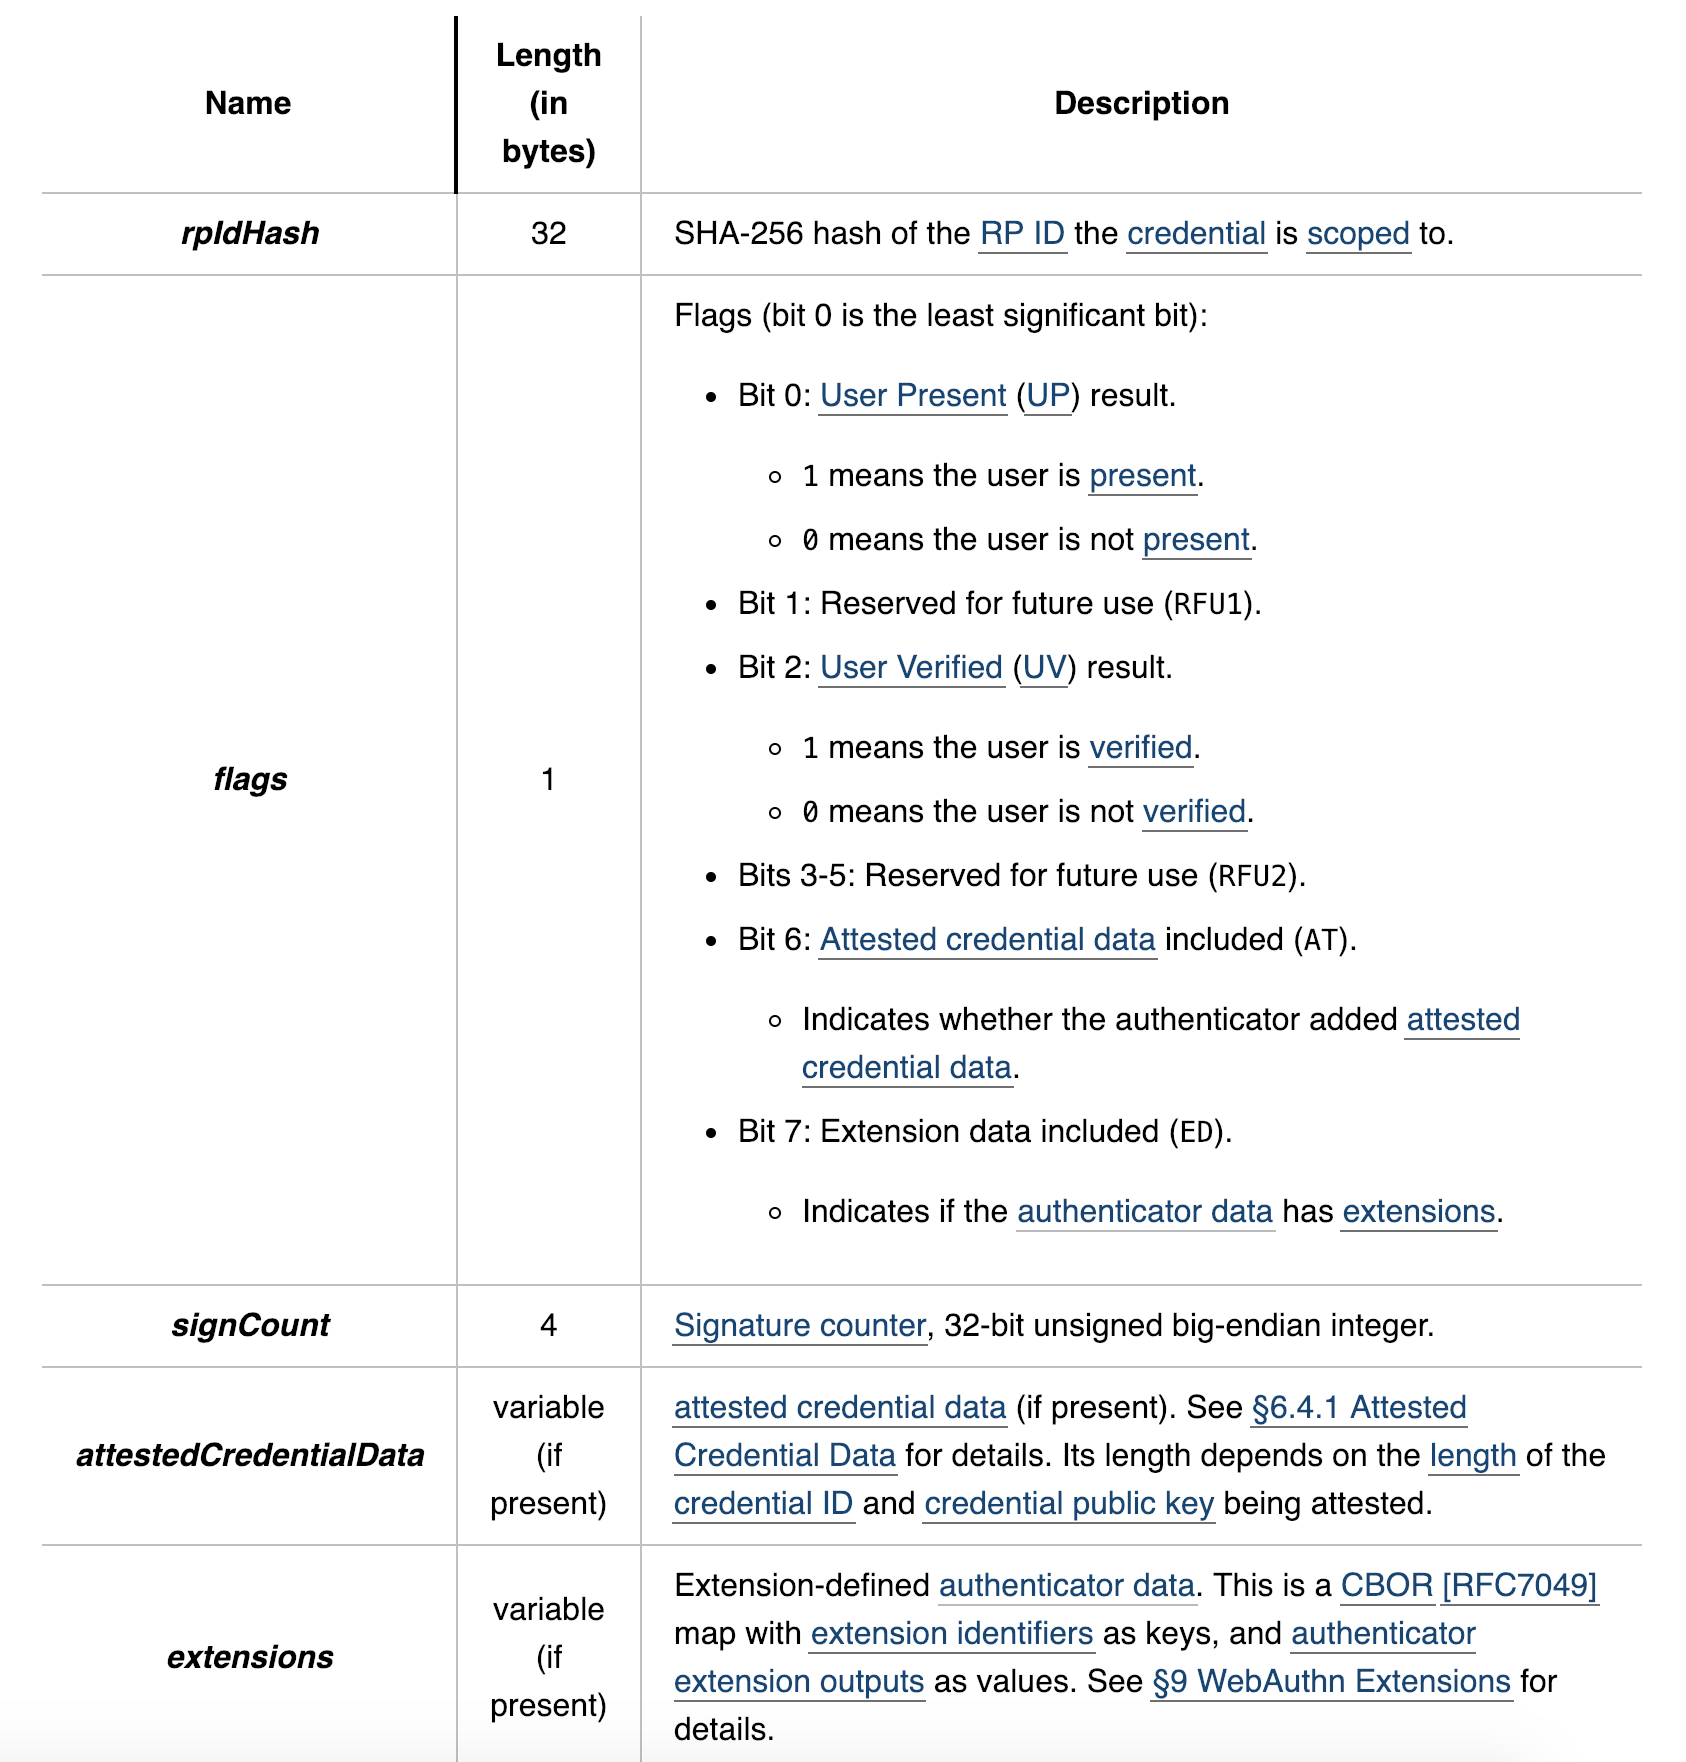
\includegraphics[width=16cm]{img/authenticatorResponseData.png}
  \centering
  \caption{Authenticator Data}
  \label{fig:authenticatorData}
\end{figure}

\begin{figure}[ht]
  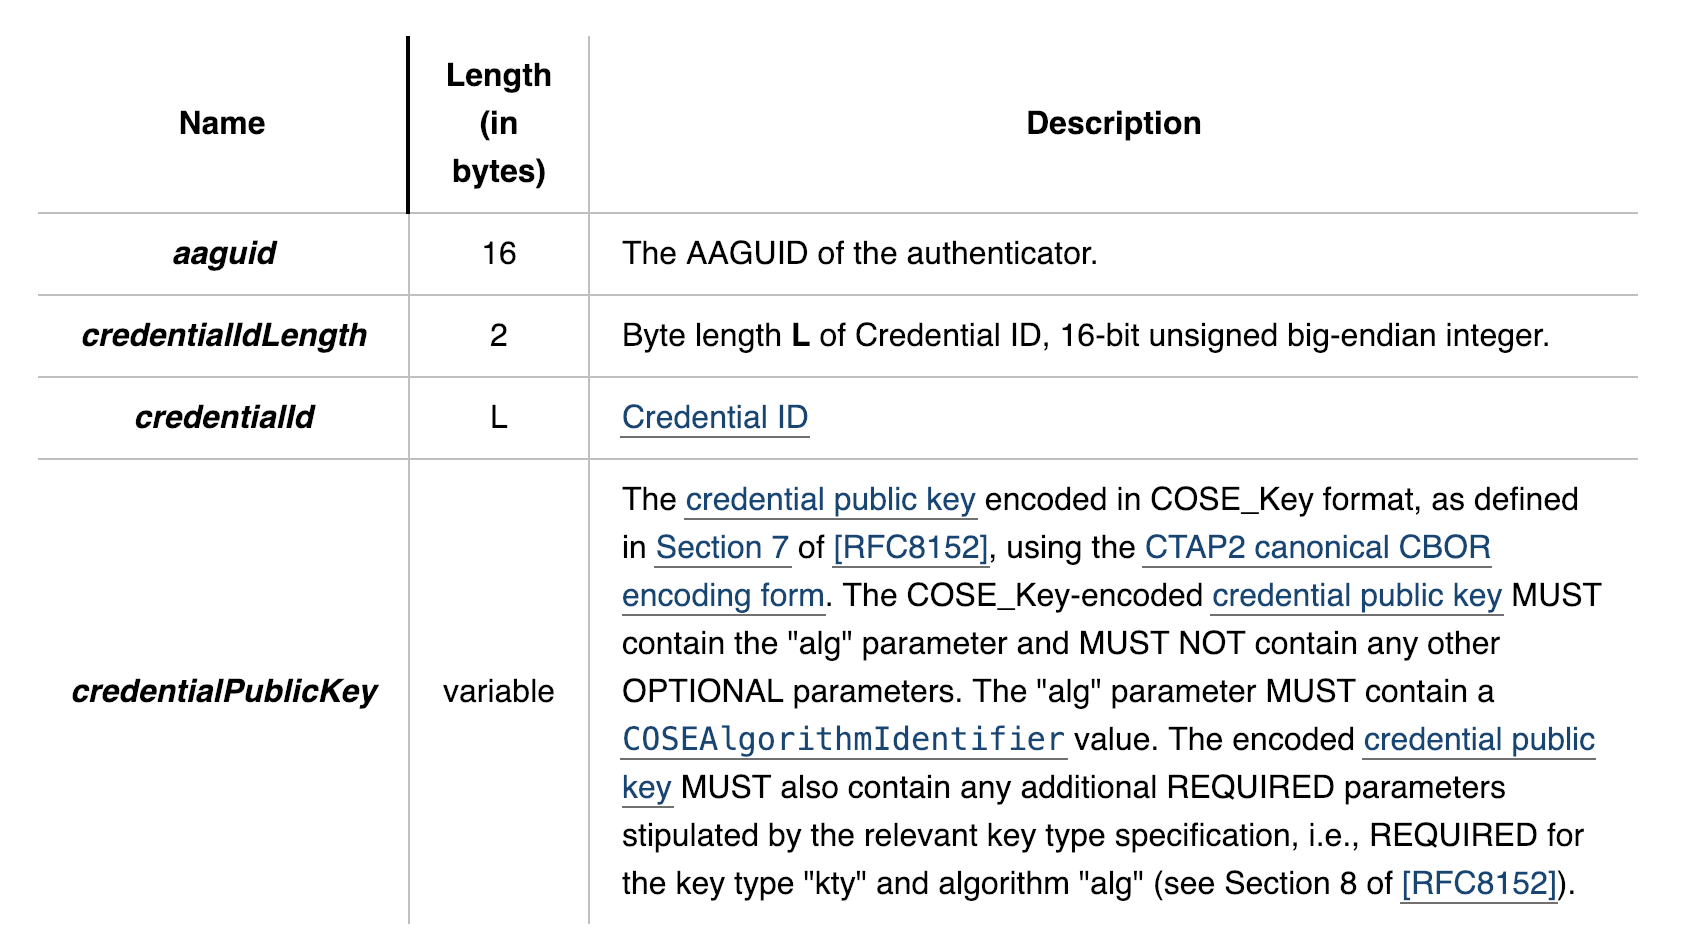
\includegraphics[width=16cm]{img/authenticatorData.png}
  \centering
  \caption{Attested Credential Data}
  \label{fig:credentialData}
\end{figure}


\clearpage

\section{Conclusion}
The \gls{fido2} standard increases the security of the end user by eliminating passwords with a \gls{mitm} resistant factor. Additionally, impersonation attacks are difficult to implement on a scale. The authenticator can be supplied by many parties which makes wide adoption easier. However, currently, the implementation of the standard for a webpage owner is probably to complexas there are not yet convenient libraries for all languages available. This needs to change if wide adoption is to be achieved. Additionally, there are not yet many \gls{fido2} authenticators available on the market. Which is a risk concerning the adoption rate.

However, the standard is considerably new and has strong support from Microsoft, where it is implemented in Windows Hello, and other big technology companies. The implementation in Windows Hello could result in many companies supplying authenticators to their employees which would lead to a higher incentive to provide web applications with \gls{fido2} support. It is crucial that other big players indeed implement the standard for core products so that it truly can replace passwords.

An exciting application of this would be within companies to replace the need for passwords at the workplace. Also, it could be used by governments in combination with an \gls{eid} to give access to specific resources by using a physical card as an authenticator. This way every citizen of a country already has access to a \gls{fido} certified authenticator which would lead to country-specific sites implementing the standard as an authentication method. 

When implementing a specific application it is important to ask some questions. Firstly, it is important to know whether multiple ways to register and authenticate need to be supported or if one way suffices. The security principle keep it simple should never be disregarded, and if it is possible to reduce the amount of code it should be done. Additionally, some thought should go into whether the user needs to be verified by the authenticator and thus turning it into a local multi factor. This rises the \gls{loa} because a stolen authenticator can't be abused without knowledge of the second factor. Additionally the certification level of the authenticators should be taken into consideration when assessing the needs.

\subsection{Further Research}

This implementation only covered the Yubikey 5 authenticator. It would be interesting to see how other authenticators react. Also, it would be interesting to see how the Yubikey 5 interacts via the \gls{nfc} interface as this implementation was only tested using the \gls{usb} interface of the authenticator. 

Additionally, it only dealt with authentication and registration. It is essential to give the user the option to add multiple authenticators to his account such that he can recover his account should he lose his key. Additionally, it is vital that the user can revoke their authenticators. This possibility should be done by giving the user the option to set a name that is relevant to him for each authenticator. He should then be able to manage those authenticators. Either adding new ones or removing existing ones. 


\clearpage

\printglossaries

\clearpage

%% Print the bibibliography and add the section to the table of content
\printbibliography[heading=bibintoc]

\end{document}
